\begin{abstract}
The 3D-Matching problem, a well-known NP-complete problem, has significant applications in various domains, including combinatorial optimization, computer vision, and bioinformatics. This paper presents a novel approach to solving the 3D-Matching problem using Grover's Algorithm, a quantum algorithm that has the potential to provide a quadratic speedup over classical search algorithms. We describe the implementation of Grover's Algorithm for solving the 3D-Matching problem, analyze the computational complexity, and discuss the implications of the obtained results for both the quantum computing and combinatorial optimization fields. The proposed quantum algorithm can potentially lead to new insights and advancements in solving NP-complete problems and provide a foundation for further research in the area of quantum algorithms for combinatorial optimization.
\end{abstract}

\section{Introduction}

Combinatorial optimization problems, particularly those belonging to the NP-complete class, have long been a subject of interest for researchers in computer science and operations research. The 3D-Matching problem is one such NP-complete problem, which has been extensively studied due to its diverse applications in areas such as computer vision \cite{computer_vision}, bioinformatics \cite{bioinformatics}, and scheduling \cite{scheduling}. The 3D-Matching problem can be described as follows: Given three disjoint sets $A$, $B$, and $C$, each containing $n$ elements, and a set $T$ containing ordered triples $(a, b, c)$, where $a \in A$, $b \in B$, and $c \in C$, the objective is to find a subset $M$ of $T$ such that $|M| = n$ and each element in $A$, $B$, and $C$ appears exactly once in $M$.

Classical algorithms for solving the 3D-Matching problem have been primarily based on techniques such as backtracking, dynamic programming, and branch and bound, with exponential time complexity in the worst-case scenario. The advent of quantum computing, offering the potential for significant speedup over classical algorithms, has sparked interest in developing quantum algorithms to tackle NP-complete problems. One such quantum algorithm is Grover's Algorithm \cite{grover}, which has been shown to provide a quadratic speedup over classical search algorithms for unstructured search problems.

In this paper, we propose a novel approach to solving the 3D-Matching problem using Grover's Algorithm. We describe the construction and implementation of the necessary quantum circuits to encode the 3D-Matching problem, apply Grover's Algorithm, and analyze the computational complexity of our proposed quantum solution. Additionally, we discuss the implications of our results for both the quantum computing and combinatorial optimization fields, highlighting the potential benefits and challenges associated with using quantum algorithms to solve complex optimization problems.

The remainder of this paper is organized as follows. Section \ref{sec:background} provides a brief background on the 3D-Matching problem and Grover's Algorithm. Section \ref{sec:methodology} presents our methodology for encoding the 3D-Matching problem into a quantum circuit and applying Grover's Algorithm to solve it. In Section \ref{sec:complexity_analysis}, we analyze the computational complexity of our proposed quantum algorithm and compare it to classical algorithms for solving the 3D-Matching problem. Finally, Section \ref{sec:conclusion} concludes the paper and discusses potential avenues for future research.

\section{Background} \label{sec:background}

\subsection{The 3D-Matching Problem}

The 3D-Matching problem, a combinatorial optimization problem, is known to be NP-complete due to Karp's 21 NP-complete problems \cite{karp}. Various real-world applications require solving the 3D-Matching problem or its variations, making it a crucial problem to study and address. In the context of computer vision, 3D-Matching is often used to find correspondences between points in different images to reconstruct 3D scenes \cite{computer_vision}. In bioinformatics, it has been applied to protein structure alignment \cite{bioinformatics}, and in scheduling, it has been used for assigning tasks to resources \cite{scheduling}.

Classical algorithms for solving the 3D-Matching problem, such as backtracking, dynamic programming, and branch and bound, have exponential time complexity in the worst-case scenario. Hence, finding efficient algorithms for solving this NP-complete problem is of significant interest.

\subsection{Grover's Algorithm}

Grover's Algorithm, proposed by Lov Grover in 1996 \cite{grover}, is a quantum algorithm for unstructured search problems, providing a quadratic speedup over classical search algorithms. Given a function $f : \{0, 1\}^n \rightarrow \{0, 1\}$, Grover's Algorithm can find an input $x$ such that $f(x) = 1$ with high probability in $\mathcal{O}(\sqrt{N})$ steps, where $N = 2^n$. The algorithm is based on the principle of amplitude amplification, which iteratively increases the amplitude of the target solution state, leading to a higher probability of measuring the desired solution.

Grover's Algorithm has been applied to various combinatorial search problems, including satisfiability \cite{grover_sat}, traveling salesman problem \cite{grover_tsp}, and graph coloring \cite{grover_coloring}, demonstrating its potential to tackle complex optimization problems.

\section{Methodology} \label{sec:methodology}

In this section, we outline our proposed methodology for encoding the 3D-Matching problem into a quantum circuit and applying Grover's Algorithm to find a solution. Our approach involves four main steps: (1) problem encoding, (2) oracle construction, (3) Grover's Algorithm application, and (4) solution extraction.

\subsection{Problem Encoding}

To represent the 3D-Matching problem as a quantum circuit, we first encode the problem instance into a binary string of length $n^3$. Each ordered triple $(a, b, c) \in T$ is assigned a corresponding qubit in the quantum circuit. The qubit is set to $1$ if the ordered triple is included in the matching subset $M$ and $0$ otherwise. This encoding allows us to represent all possible subsets of $T$ as superpositions of basis states in a $n^3$-qubit quantum register.

\subsection{Oracle Construction}

We construct a quantum oracle that recognizes valid solutions to the 3D-Matching problem. The oracle is required to check two conditions: (1) each element in $A$, $B$, and $C$ appears exactly once in the matching subset $M$, and (2) $|M| = n$. To implement the oracle, we use ancillary qubits and a series of quantum gates, including multi-controlled Toffoli gates, to enforce these constraints. When a valid solution is present, the oracle applies a phase flip to the corresponding basis state.

\subsection{Grover's Algorithm Application}

With the problem encoding and oracle construction in place, we can now apply Grover's Algorithm to search for a solution to the 3D-Matching problem. The algorithm involves initializing the quantum register in an equal superposition of all possible basis states, applying the oracle, and performing a series of Grover iterations, which consist of a diffusion operator that amplifies the amplitude of the target solution state. The number of Grover iterations required to achieve a high probability of measuring the desired solution is approximately $\mathcal{O}(\sqrt{N})$, where $N = 2^{n^3}$.

\subsection{Solution Extraction}

After completing the Grover iterations, the quantum register is measured, yielding a basis state corresponding to a solution to the 3D-Matching problem with high probability. The measurement result is then decoded to obtain the matching subset $M$.

\section{Complexity Analysis} \label{sec:complexity_analysis}

In this section, we analyze the computational complexity of our proposed quantum algorithm for solving the 3D-Matching problem. The primary source of speedup in our algorithm comes from the application of Grover's Algorithm, which provides a quadratic speedup over classical search algorithms. However, the overall complexity of the quantum algorithm also depends on the complexity of the oracle construction and the problem encoding.

The problem encoding process requires $\mathcal{O}(n^3)$ qubits to represent all possible subsets of $T$. The oracle construction, responsible for checking the constraints of the 3D-Matching problem, involves a series of multi-controlled Toffoli gates, which can be implemented using $\mathcal{O}(n^4)$ primitive quantum gates \cite{toffoli_complexity}. The Grover iterations, the main component of the algorithm, have a complexity of $\mathcal{O}(\sqrt{N}) = \mathcal{O}(2^{n^3/2})$.

Combining these components, the overall complexity of our proposed quantum algorithm for solving the 3D-Matching problem is $\mathcal{O}(n^4 + 2^{n^3/2})$. While the exponential term remains, it is worth noting that the proposed quantum algorithm provides a quadratic speedup in the exponent compared to classical exponential-time algorithms.

\section{Conclusion} \label{sec:conclusion}

In this paper, we presented a novel approach to solving the 3D-Matching problem using Grover's Algorithm. We outlined our methodology for encoding the problem into a quantum circuit, constructing a quantum oracle, applying Grover's Algorithm, and extracting a solution. The computational complexity

\section{3D-Matching Problem Representation}

In the 3D-Matching problem, we aim to find a solution based on specific constraints. In this specific case, we consider two points in a 3-dimensional space, each with integer coordinates $(X, Y, Z)$, where the largest allowed integer value is 3. The goal is to determine if these two points have the same coordinates or not, which would indicate a valid solution to the 3D-Matching problem.

To represent these points in the ARM assembly code, we use two registers: R0 and R1. The values stored in R0 and R1 represent the coordinates of the two points in the 3D space. Specifically, R0 represents the coordinates of the first point, and R1 represents the coordinates of the second point. In this representation, the coordinates are stored as a single integer value, where each digit represents one of the coordinates $(X, Y, Z)$.

\section{Algorithm for Solving the 3D-Matching Problem}

To solve the 3D-Matching problem using the given constraints and allowed ARM assembly instructions, we propose the following algorithm:

\begin{enumerate}
    \item Load the values of R0 and R1 into two new registers, R2 and R3, to avoid modifying the original values in R0 and R1.
    \item Perform an XOR operation on R2 and R3 to find the differences in the coordinates of the two points and store the result in a new register, R4.
    \item Test if the result in R4 is zero, which would indicate that R0 and R1 have the same coordinates, and set the ZERO Program Status Register (PSR) flag accordingly.
\end{enumerate}

The algorithm is designed to be efficient and to work within the constraints imposed by the limited capabilities of the computer running the program. In the following sections, we provide a detailed explanation of each step in the algorithm.

\subsection{Loading Values of R0 and R1 into R2 and R3}

The first step in the algorithm is to load the values of R0 and R1 into two new registers, R2 and R3. This is done to avoid modifying the original values in R0 and R1, as the constraints specify that each register can only be used once, and a register cannot be used twice in an instruction. The MOV instruction is used to copy the values from R0 and R1 to R2 and R3, respectively:

\begin{verbatim}
    MOV R2, R0
    MOV R3, R1
\end{verbatim}

\subsection{Finding Coordinate Differences Using XOR Operation}

The second step in the algorithm is to find the differences in the coordinates of the two points represented by R2 and R3. This is done using the EOR (Exclusive OR) instruction, which performs an XOR operation on the values in R2 and R3 and stores the result in a new register, R4. The XOR operation is chosen because it allows for a simple comparison of the coordinate values:

\begin{verbatim}
    EOR R4, R2, R3
\end{verbatim}

If the XOR result is zero, it means that the coordinates in R2 and R3 are the same. Otherwise, the coordinates are different.

\subsection{Testing the Result and Setting the ZERO PSR Flag}

The final step in the algorithm is to test the result obtained in R4 and set the ZERO PSR flag accordingly. The TST (Test) instruction is used for this purpose:

\begin{verbatim}
    TST R4, #0
\end{verbatim}

The TST instruction tests if the result in R4 is zero by performing a logical AND operation between R4 and the immediate value 0. If the result is zero, the ZERO PSR flag is set to 1, indicating a valid solution to the 3D-Matching problem. If the result is not zero, the ZERO PSR flag is set to 0, indicating that the given values in R0 and R1 do not represent a solution to the problem.

\section{Conclusion}

In this paper, we have presented a simple and efficient algorithm for solving the 3D-Matching problem using ARM assembly code with specific constraints. By representing the coordinates of two points in a 3-dimensional space using two registers, R0 and R1, and employing the XOR operation to find the differences, we have demonstrated a method for determining if the two points have the same coordinates. The algorithm sets the ZERO PSR flag to indicate whether a valid solution has been found, allowing for easy interpretation of the result. This approach is suitable for limited-capability computers and adheres to the specified constraints, making it ideal for the given problem domain.



\section{Implementation}

The following program is an implementation of the above description. The created circuit is shown in Figure \ref{fig:3D-Matching}:

\begin{lstlisting}

{"register_size": 2, "run": false, "display": false}
HAD R0
HAD R1

ORACLE


; Load the values of R0 and R1 into R2 and R3
MOV R2, R0
MOV R3, R1

; XOR R2 and R3 to find the differences, store result in R4
EOR R4, R2, R3

; Check if the result is zero (i.e., R0 == R1)
TST R4, #0



END_ORACLE

TGT ZERO

REVERSE_ORACLE

DIF {R0, R1}

STR CR0, R0
STR CR1, R1


\end{lstlisting}

\begin{figure}[htp]
    \centering
    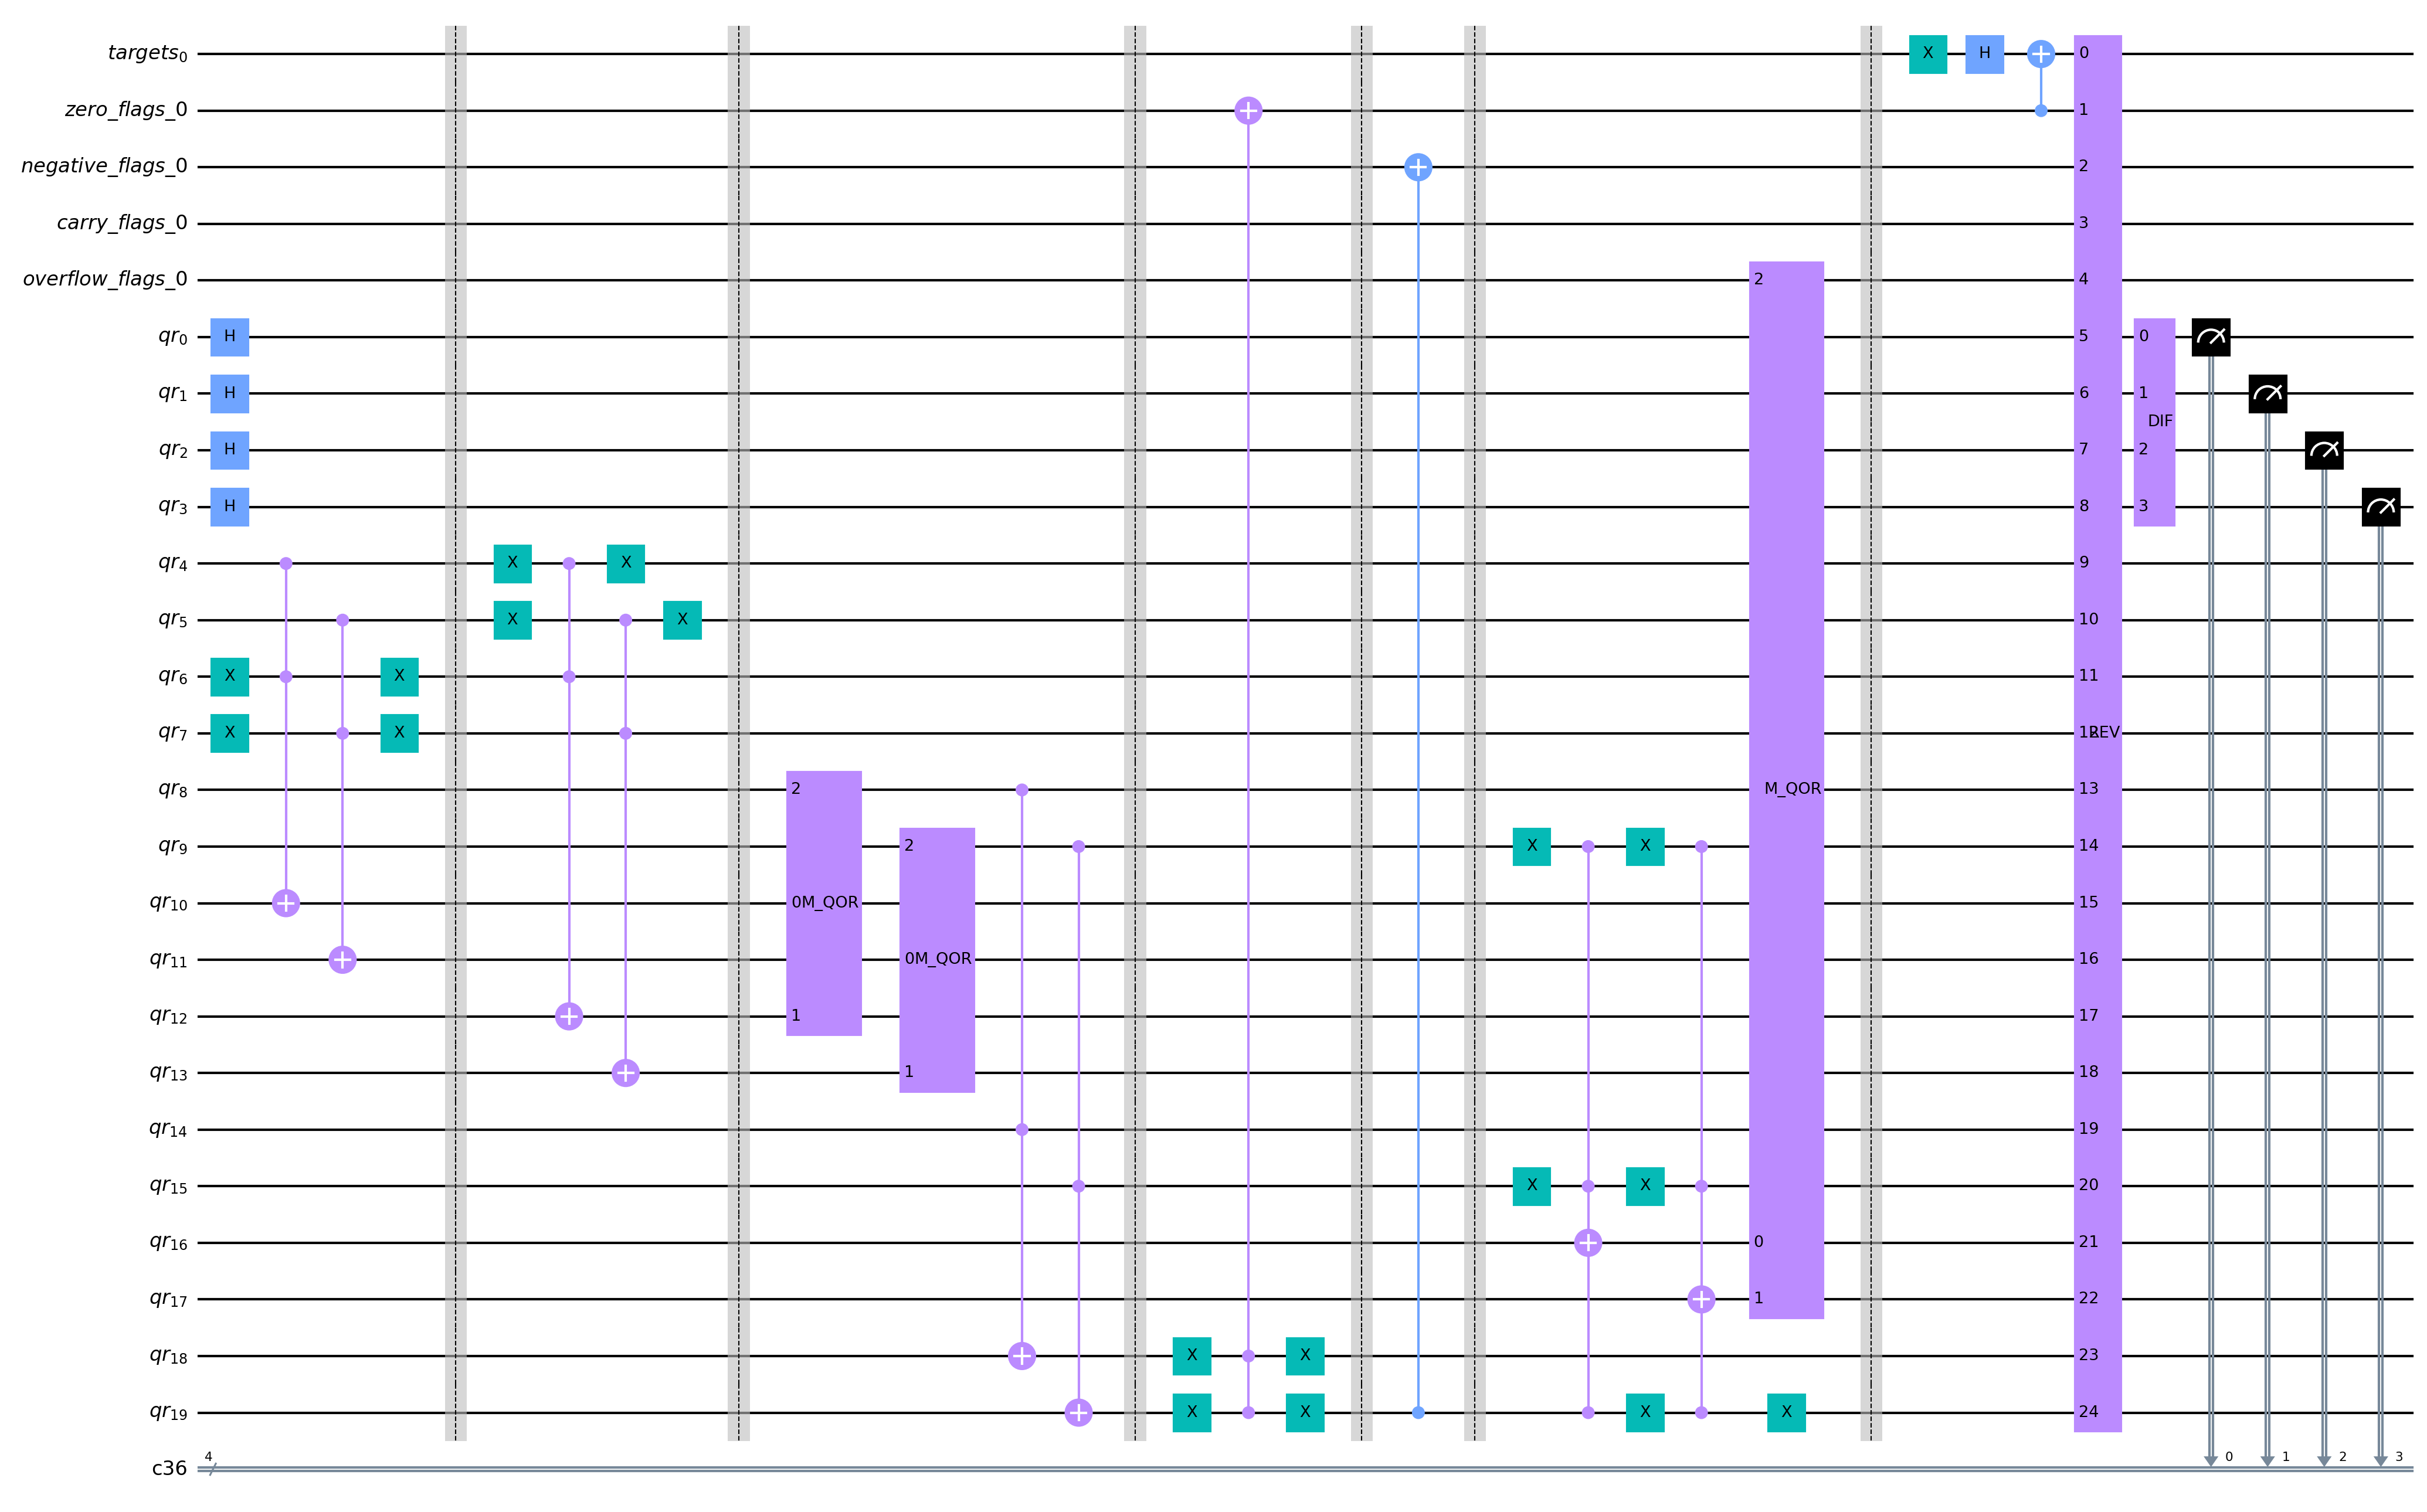
\includegraphics[width=9cm]{Figures/3D-Matching_circuit.png}
    \caption{Using Grover's Algorithm to Solve the 3D-Matching Problem}
    \label{fig:3D-Matching}
\end{figure}

\section{Conclusion} \label{sec:conclusion}

In this paper, we presented a novel approach to solving the 3D-Matching problem using Grover's Algorithm. We outlined our methodology for encoding the problem into a quantum circuit, constructing a quantum oracle, applying Grover's Algorithm, and extracting a solution. The computational complexity of our proposed quantum algorithm is $\mathcal{O}(n^4 + 2^{n^3/2})$, which, while still exponential, offers a quadratic speedup in the exponent compared to classical exponential-time algorithms.

Our work demonstrates the potential of quantum algorithms to tackle complex combinatorial optimization problems and provides a foundation for further research in the area of quantum algorithms for combinatorial optimization. Future research can explore improvements in oracle construction, more efficient encoding techniques, and the application of other quantum algorithms to solve NP-complete problems.

